
\documentclass{article} % For LaTeX2e
\usepackage{kenzo,times}
\usepackage{graphicx}
\usepackage{placeins}
\usepackage{booktabs}
\usepackage{chngcntr}

% Optional math commands from https://github.com/goodfeli/dlbook_notation.
\input{math_commands.tex}

\usepackage{hyperref}
\usepackage{url}

\title{Title}

\author{Fernando K.I. Fugihara \\
Universidade Estadual de Campinas – UNICAMP\\
Campinas, SP, Brazil, 13083-896 \\
\texttt{f205067@dac.unicamp.br} \\
}

% The \author macro works with any number of authors. There are two commands
% used to separate the names and addresses of multiple authors: \And and \AND.

\newcommand{\fix}{\marginpar{FIX}}
\newcommand{\new}{\marginpar{NEW}}

\kenzofinalcopy % Uncomment for final version
\begin{document}

\begin{titlepage}
    \centering

    % Logos
    \begin{figure}[t]
        \centering
        \begin{minipage}{0.4\textwidth}
            \centering
            
\includegraphics[width=0.8\textwidth]{figures/logo_nipe.png}
        \end{minipage}
        \hfill
        \begin{minipage}{0.3\textwidth}
            \centering
            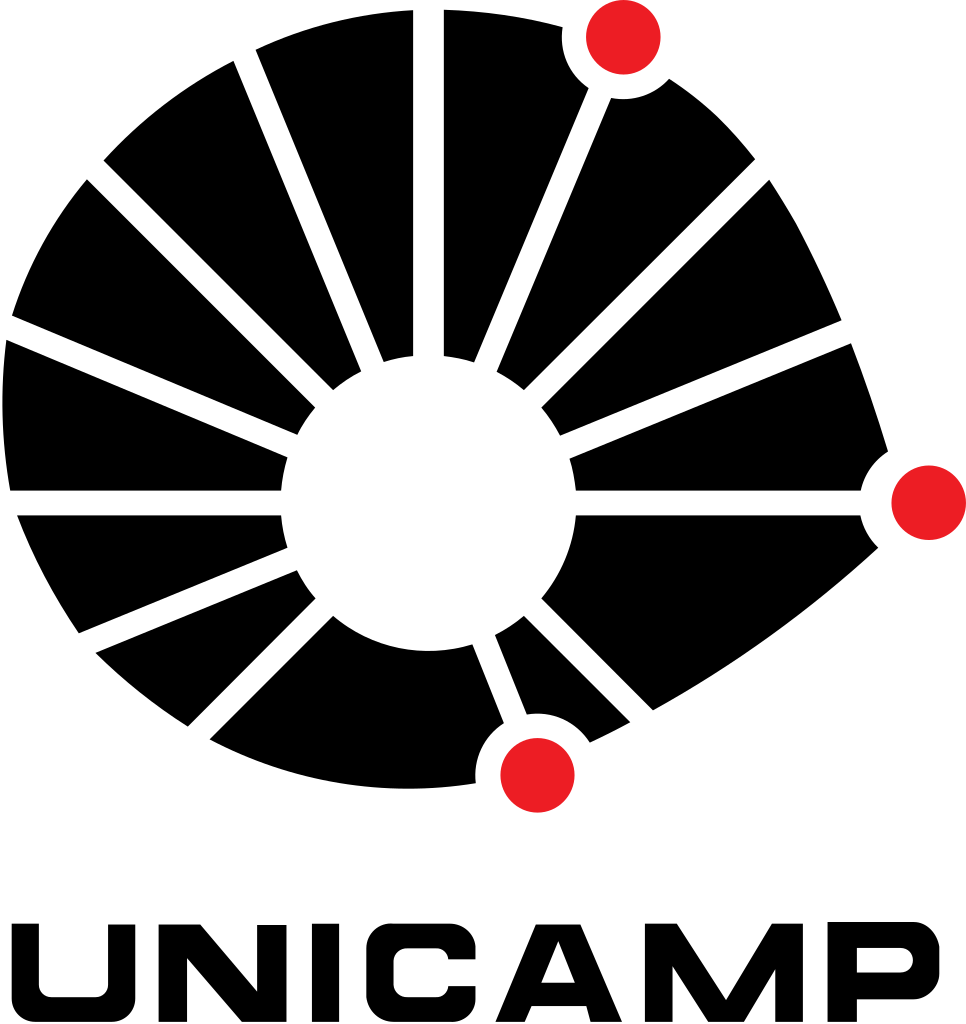
\includegraphics[width=0.8\textwidth]{figures/unicamp.png}
        \end{minipage}
    \end{figure}

    \vspace{1cm}

    {\Large \textbf{Research Internship Abroad (BEPE/FAPESP)}}\\[1cm]

    {\LARGE \textbf{Remote Sensing Anomaly Detection in Time-Series Imagery}}\\
    {\LARGE \textbf{and Application Development in the Agricultural Context}}\\[1.5cm]

    {\large Process: 2025/22483-0}\\[0.5cm]

    {\large Final Report: December 01, 2025 -- March 01, 2026 (3 months)}\\[3cm]

    \begin{flushright}
        {\large \textbf{Brazil Advisor:} Dr. Rubens Augusto Camargo Lamparelli}\\
        {\large \textbf{UK Supervisor:} Dr. Jefersson Alex dos Santos}\\
        {\large \textbf{UK Co-Supervisor:} Prof. Po Yang}\\
        {\large \textbf{Fellow:} Fernando Kenzo Imami Fugihara}
    \end{flushright}

    \vfill

    {\large Campinas, SP}\\
    {\large 2026}

\end{titlepage}


\begin{abstract}
The use of plastic in agriculture has increased significantly in recent years, bringing both benefits and environmental challenges. While agricultural plastics improve crop yields and resource efficiency, they also lead to the accumulation of plastic waste in rural areas. Remote Sensing (RS) data, combined with advanced machine learning and computer vision techniques, provide an effective means to monitor plasticulture dynamics. Therefore, this research internship aims to explore RS anomaly detection (RSAD) techniques in time-series imagery and apply them to agricultural monitoring, particularly in detecting subtle cases that involve spectral changes such as material deterioration and pest-related disturbances. Therefore, I’ll join researchers at the University of Sheffield to learn RSAD techniques in the agriculture context and then explore whether they can be applied in plasticulture. In parallel, I’ll collaborate with researchers at the University of Sheffield and contribute to the PEZEGO pest-management app. The internship will provide hands-on experience in scalable application design, app optimization, and model integration, which can enhance our ongoing application, GeoHuman. The University of Sheffield was chosen due to its internationally recognized expertise in application development, machine learning, computer vision, and remote sensing. This experience will strengthen our project in Brazil by improving the accuracy and scalability of agricultural monitoring systems. Upon my return, I will disseminate the knowledge gained through workshops and collaborative activities with my research group at UNICAMP to fos	ter innovation and capacity building in remote sensing applications.

\end{abstract}

    
\section{Introduction}

    The use of plastic in agriculture, commonly referred to as Plasticulture \citep{dubois1978plastics,levin2007remote}, has increased steadily in recent years \citep{perilla2019high}. According to \cite{sintim2017biodegradable}, the global annual usage of plastic films in land-based farming is estimated at 7.4 million tons, mostly from greenhouses and mulching \citep{fao2021assessment}. As plastics become increasingly prevalent in rural areas, concerns about agricultural plastic waste (APW) are escalating (Figure 1). Plastic waste has gained worldwide attention, prompting discussions among numerous countries and international organizations about potential solutions. These conversations include various aspects, including the use of plastic in agriculture \citep{ec2019circular,fao2021assessment,hofmann2023plastics,unep2018mapping,unep2022resolution}. Therefore, mapping plasticulture sites is crucial, and one effective method involves using Remote Sensing (RS) data combined with advanced computer vision (CV) algorithms trained to classify RS images. 


    \begin{figure}[!ht]
        \centering
        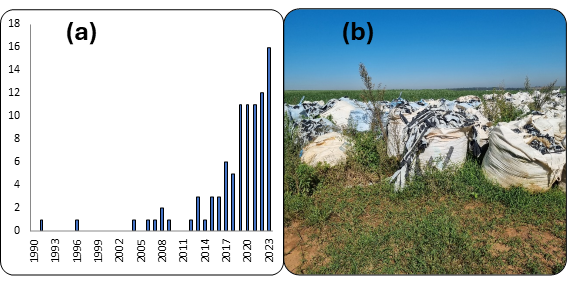
\includegraphics[width=0.7\textwidth]{figures/Fig1_nerc-fapesp.png}
        \caption{Growth in publications about agri-plastic remote detection. (b) APW deposited on a farm in Brazil awaiting correct disposal. Sometimes producers face difficulties finding someone to collect the plastic. Search in Web of Science on October 11th of 2023 with the query TS= ((agricultural plastic OR agro-plastic OR agroplastic OR agri-plastic OR agriplastic OR plasticulture) AND (remote sensing OR classification OR mapping OR detection) AND (greenhouse OR mulch*)).}
        \label{fig:scholar}
    \end{figure}
    \FloatBarrier


    Monitoring plasticulture requires careful attention during critical crop stages, especially those involving pest control and the post-harvest period, when the plastic cover reappears in RS imagery. These transitions can cause spectral variations detectable in RS data \citep{dubucq2020remote,holt2025hyperspectral}. Examples of such variations include those caused by the temporary use of pest-protection nets (Figure 
    \ref{pestnet}a) and the reappearance or gradual change of plastic (Figure \ref{pestnet}b). Over time, factors such as sunlight exposure, temperature changes, and mechanical stress may also alter the material properties of agricultural plastics, subtly impacting their spectral signatures \citep{dubucq2020remote}. Additionally, the use or removal of pest-control nets can also alter the scene’s reflectance, introducing spectral variations detectable in RS data, verified through our field observations. In this context, Remote Sensing Anomaly Detection (RSAD) offers a valuable framework for identifying these subtle and unexpected spectral deviations from standard temporal patterns, thereby facilitating the continuous monitoring of plasticulture activities and related farming practices \citep{kwon2005kernel}.


    \begin{figure}[!ht]
        \centering
        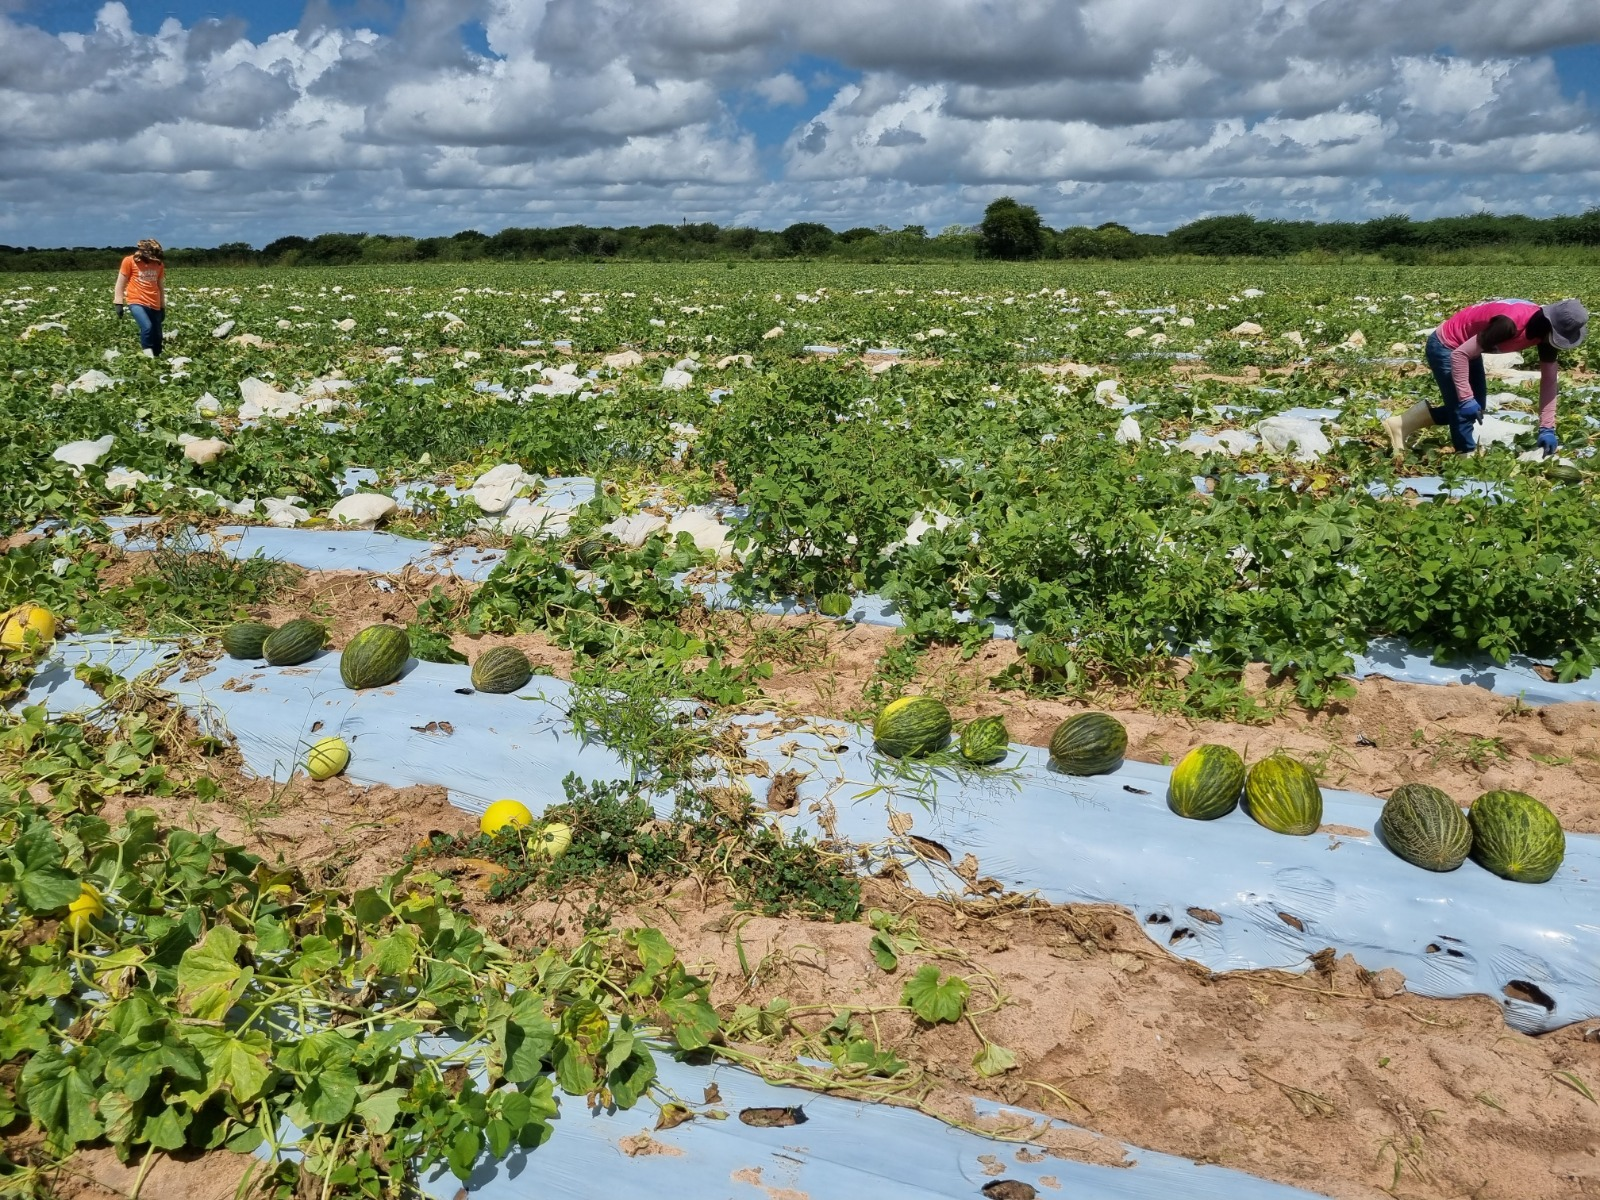
\includegraphics[width=0.7\textwidth]{figures/1000062840.jpg}
        \caption{Subtle dynamics of agricultural plastic use in Mossoró, RN, Brazil. a) The temporary use of a pest-control net to shield the crops. b) The reappearance and presence of the underlying plastic mulch after harvest. Photographs taken during a field visit by our research group.}
        \label{pestnet}
    \end{figure}
    \FloatBarrier

    RSAD has been widely studied \citep{racetin2021systematic,guo2016novel} and successfully applied to various domains, including environmental monitoring \citep{guo2016novel}, urban mapping \citep{rejas2016hyperspectral}, and disaster detection \citep{anand2022anomaly}. The University of Sheffield hosts a leading group in Anomaly Detection (AD), and through our discussions with them, we identified a research theme of mutual interest. Then I will explore the potential of applying RSAD techniques to monitor the plasticulture cycle using time series data, particularly to detect subtle deviations such as plastic deterioration and pest control practices.


    AD models that rely on RS imagery present significant challenges for agricultural detection due to variable illumination, heterogeneous and complex landscapes, and seasonal or phenological variations \citep{fu2025lightweight}. A crucial step for applying RSAD techniques to time-series data is the effective preprocessing of satellite imagery, which ensures that the model outputs are reliable and accurate. One of the problems is the cloud cover, which obscures or contaminates surface reflectance and is especially evident in long-term data \citep{gawlikowski2022explaining,king2013spatial,wen2001impact}. In my ongoing research in Brazil, I have worked extensively on preprocessing techniques, including cloud masking, multimodal fusion, and geographic target analysis, to improve the detection of agricultural plastics. Building on this background, engaging with researchers at Sheffield will allow me to integrate preprocessing with advanced RSAD approaches. 


    One of the main challenges the circular economy group faced was collecting sufficient data to train CV algorithms for effective plasticulture monitoring. Given this context and considering the limited funding and manpower for field data collection, our team developed a web-based application (GeoHuman) featuring an intuitive user interface to facilitate rapid user adoption \citep{bodi1992intuitive}. Our app, currently in development, generates high-quality RS-labeled datasets by applying CV models and preprocessing techniques in a pipeline. This work is part of the FAPESP-Braskem project (2021/052251-8). However, the application still faces significant challenges, including the need to scale efficiently to support a large number of users, reduce model prediction time, and support only local deployment. These bottlenecks currently hinder the system's usability for broader agricultural applications.


    Considering the current challenges of our research in Brazil, I intend to establish a collaboration with researchers at the University of Sheffield, who have extensive experience in developing software applications for agricultural monitoring and management. Working with them will allow me to learn advanced methodologies in scalable system design, mobile app development, and model optimization. By acquiring these techniques and incorporating them into the ongoing development of our application, I will overcome the existing limitations and significantly enhance its efficiency, scalability, and quality in Brazil.


    This research internship abroad has one main goal: to increase knowledge through collaboration with researchers at the University of Sheffield, focusing on learning RSAD techniques and developing applications. We will explore whether RSAD in time series can be used in the agricultural context. These techniques could be applied in plasticulture, particularly in mulched crops. I’ll also apply software development techniques to our app, GeoHuman. Therefore, this project aims to improve my skills in these areas and gain hands-on experience with a different team. The graphical abstract of the project is presented in Figure 3.

    \begin{figure}[!ht]
        \centering
        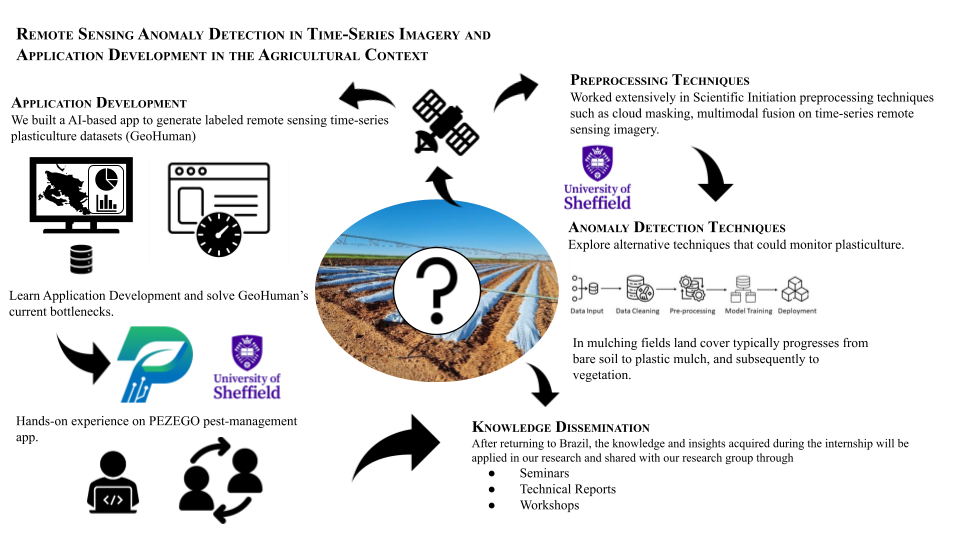
\includegraphics[width=1\textwidth]{figures/graphical_abstract.png}
        \caption{Graphical Abstract of BEPE.}
        \label{fig:graphical_abstract}
    \end{figure}
    \FloatBarrier

    \section{Methodology}
        At the University

        Figure \ref{fig:abstract} illustrates the conceptual framework of FAW infestation detection. We first detect the anomaly in S2 time-series (FAW infestation), then we model an anomaly detection algorithm to identify such events, and  finally we can create alerts for farmers to take action.

        \begin{figure}[!ht]
            \centering
            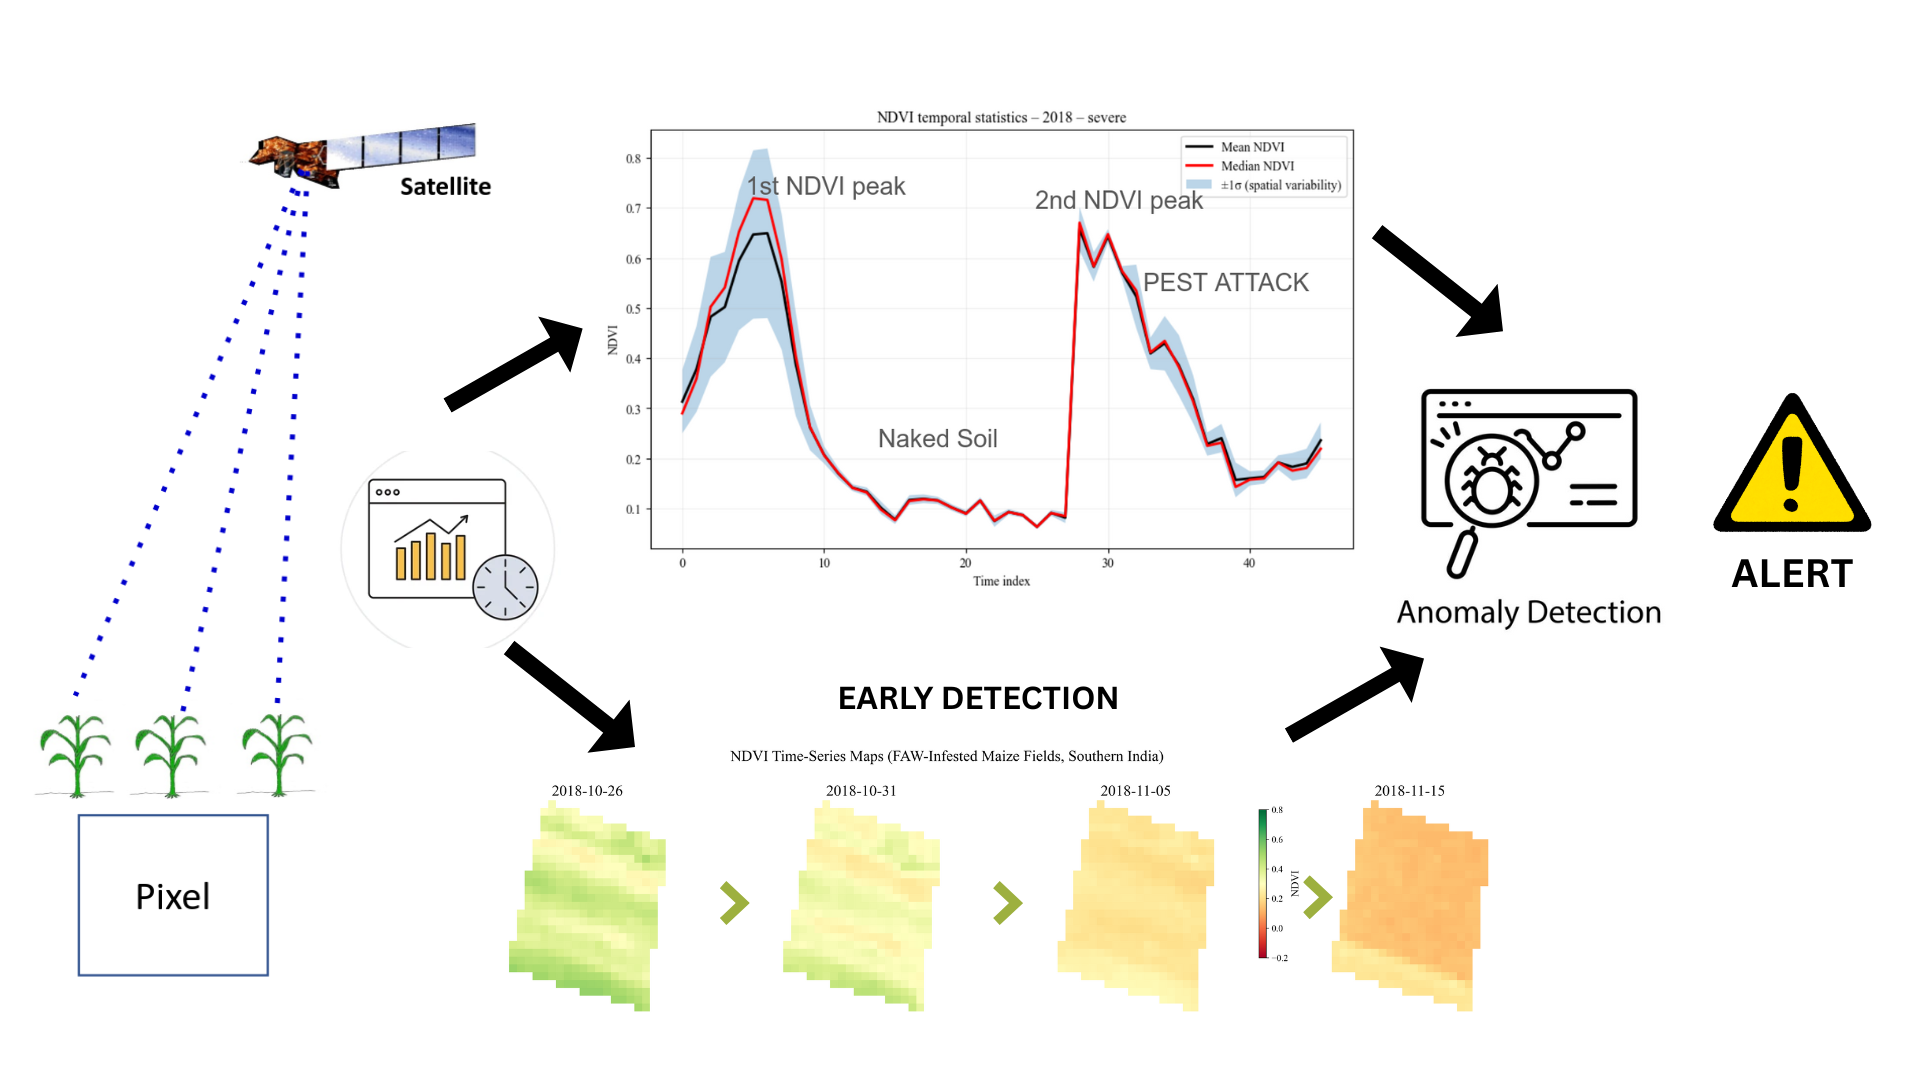
\includegraphics[width=1\textwidth]{figures/overview.png}
            \caption{Conceptual framework of FAW infestation detection using Sentinel-2 time-series analysis.}
            \label{fig:abstract}
        \end{figure}
        \FloatBarrier

    \subsection{Data and Study Regions}
        This research utilizes Harmonized Sentinel-2 (S2) Level-2A surface reflectance imagery, accessed through Google Earth Engine (GEE). The Copernicus Sentinel-2 mission consists of two polar-orbiting satellites (2A and 2B) operating in sun-synchronous orbit at 786 km altitude, phased 180° apart.

        \subsubsection{Kurnool and Gadwal Districts, Southern India}

            \cite{prabhakar2022detecting} conducted field surveys in Kurnool and Gadwal districts of Southern India to map FAW infestations in maize crops (sorghum). In his field surveys, the author mapped the regions as healthy, low, medium, and severe infestation levels. Based on that,we selected one field classified as severe infestation for our proof of concept. The \cite{prabhakar2022detecting} field survey confirmed that the FAW infestation occurred between October 26, 2018 and November 15, 2018. Figure \ref{fig:study_area_india} shows the agricultural landscape characteristics of these districts.

            \begin{figure}[!ht]
                \centering
                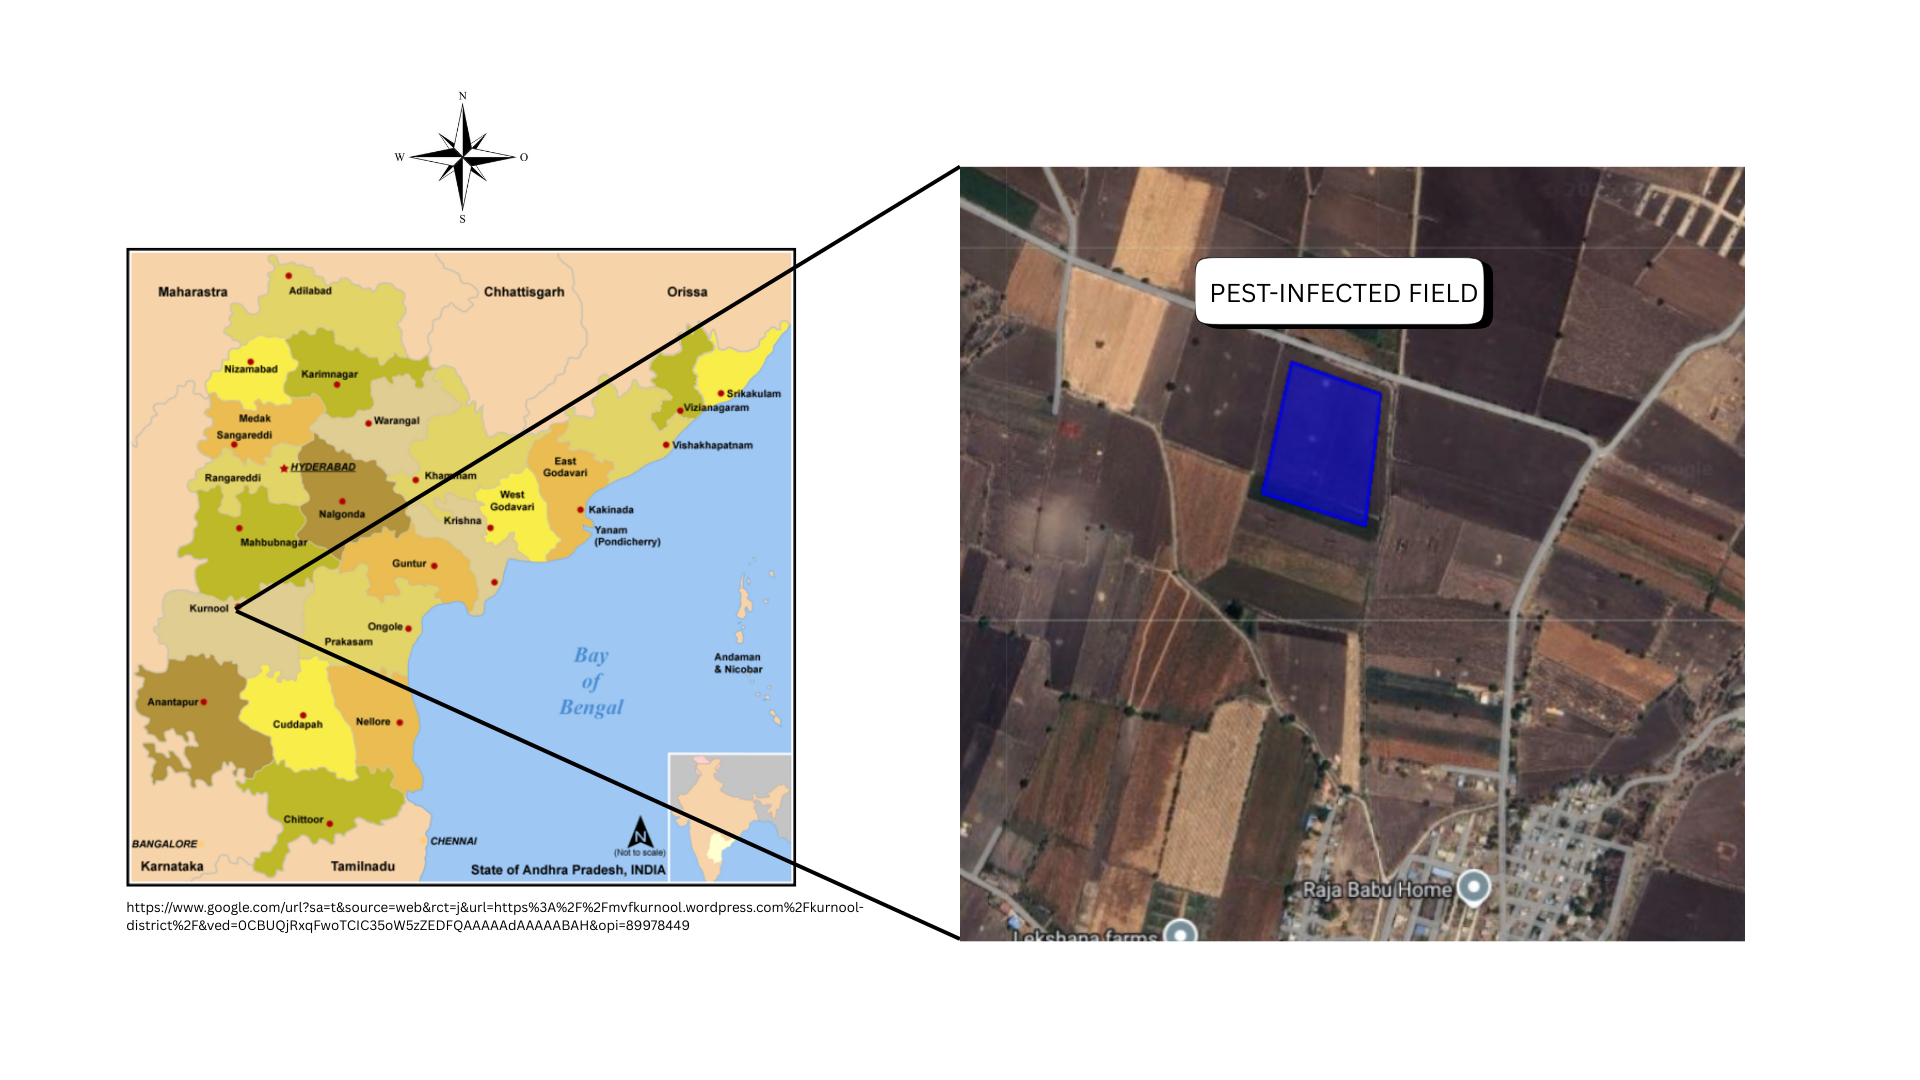
\includegraphics[width=1\textwidth]{figures/study_area_india.png}
                \caption{Kurnool and Gadwal districts, Southern India, showing maize cultivation areas.}
                \label{fig:study_area_india}
            \end{figure}
            \FloatBarrier

            \subsubsection{Ejura, Ghana, West Africa}

            Figure \ref{fig:study_area_ghana} presents the diverse agricultural landscape of Ejura, where \cite{bilintoh2019remote} conducted field validation from April to September 2017 to confirm FAW infestations. Located in the Ashanti Region's transition zone, the district features a mix of grassland and woodland with an annual rainfall of 1,200--1,500 mm and average temperatures between 26.4°C and 27.5°C. Agriculture is the primary livelihood for the population of 85,000, with a landscape dominated by commercial maize and watermelon alongside subsistence crops like yam, cassava, and plantain. The region's high vulnerability to pests is exacerbated by its complex farming systems, where frequent intercropping and crop rotation.

            \begin{figure}[!ht]
                \centering
                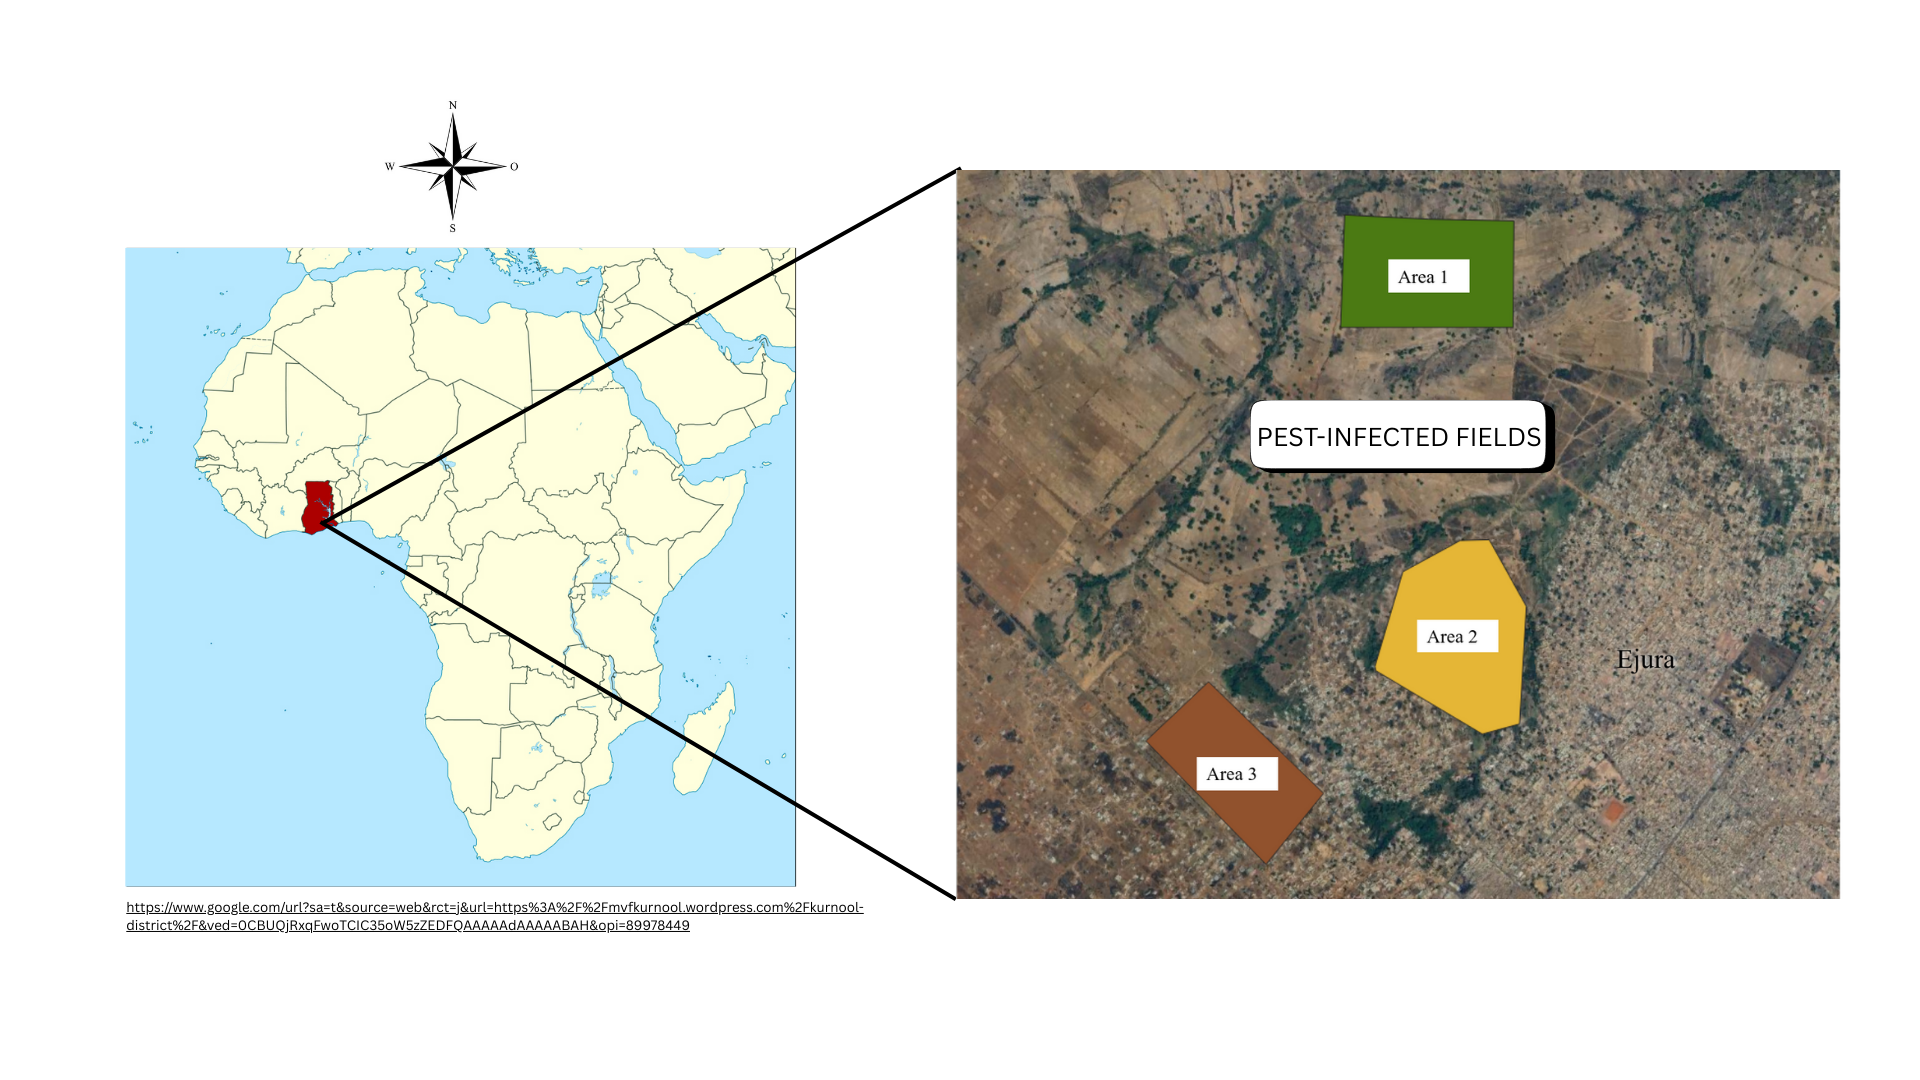
\includegraphics[width=1\textwidth]{figures/study_area_ghana.png}
                \caption{Ejura study region, Ghana, West Africa, showing diverse crop systems.}
                \label{fig:study_area_ghana}
            \end{figure}
            \FloatBarrier

    \subsection{Time-Series Analysis}
        \subsubsection{Time-Series representation}
            In this study, we used a Univariate Time-Series (UTS) representation, where each field is represented by a single spectral index (e.g., NDVI) observed over time. This approach focuses on capturing the temporal evolution and phenological patterns of a single vegetation characteristic. Given a field observed over t timestamps, the series X is defined as a sequence of scalar values:

            \begin{equation}
            X = (x_1, x_2, \ldots, x_t)
            \end{equation}

            Where each $x_i$ represents the value of the spectral index at time $i$. Unlike multivariate approaches, this representation simplifies the analysis by focusing on the variance and trend of a single physical parameter to detect anomalies or growth stages.

        \subsubsection{Time Series Components}
        An important technique when using time series is that we can divide the data into four components: the Trend, the Seasonality, the Cyclicity and the Noise. Depending on the problem and context, these components can be analysed separately or combined to better understand the underlying patterns. In agriculture, seasonality and cyclicity are often the most informative, as crop growth and environmental conditions follow recurring patterns. In contrast, in financial markets, the trend component typically provides more insight than the others, especially for long-term analysis. The following sections provide the definitions of each component.

        \subsubsection{Anomalies in Time-Series}
            According to Hawkings et al (1980) an anomaly is a data point or sequence that deviates from the general data distribution. In a time-series dataset, only a small fraction contains anomalies, where the majority of the data points follow expected patterns. There are different types of anomalies in time-series including global, trend, cycle and seasonal.

            In our context, the type of anomaly that we expect to find is the cycle anomaly, which is a deviation from the expected cyclic pattern. For example, in agricultural monitoring, a cycle anomaly could indicate an unexpected drop in vegetation health during a period when crops are typically thriving, potentially signaling pest infestations or disease outbreaks.
        
        \subsubsection{Time Series Smoothing}
        Time series smoothing is a technique used to reduce noise and improve data quality, making underlying patterns easier to analyse. In this study, we applied Triple Exponential Smoothing (TES), which effectively models the level, trend, and seasonality components commonly present in agricultural satellite time series. \ref{appendix1} presents different smoothing techniques and its mathematical formulations.

    \subsection{Preprocessing Sentinel-2 Imagery}
        In remote-sensing data, there is a lot of different informations that deviate from normality, such as sensor noise, atmospheric effects, cloud cover, seasonal variations, and landscape complexity \citep{fu2025lightweight}. The most meaningful deviations are usually those that are significantly different from the norm.

        Preprocessing is a crucial step in machine learning and data pipelines \citep{tawakuli2025survey}. It employs various techniques to ensure that the data fed into a model is clean, consistent, and informative, which directly influences its performance and reliability \citep{zheng2021improved}. This is especially important in RSAD modeling. In RS imagery, data quality can be compromised by factors such as Earth's geometric effects resulting from its curvature and rotation, atmospheric conditions like cloud cover, sensor noise, seasonal variations, and landscape complexity \citep{fu2025lightweight}.

        \subsubsection{Spectral Indices}

            Studies from \cite{bilintoh2019remote} and \cite{prabhakar2022detecting}, have demostrated the effectiveness of using spectral indices in anomaly detection. They used indices such as the Normalized Difference Vegetation Index (NDVI), the Enhanced Vegetation Index (EVI) and the Leaf Area Index (LAI). Table \ref{tab:veg_indices} presents the spectral indices used in this research, along with their mathematical formulations.

            \begin{table}[ht]
            \centering
            \caption{Spectral vegetation indices and corresponding equations using Sentinel-2 bands.}
            \label{tab:veg_indices}
            \renewcommand{\arraystretch}{1.4}
            \small
                \begin{tabular}{p{3cm} p{3cm} p{3cm}}
                \textbf{Index} & \textbf{Equation} & \textbf{Reference} \\
                \hline
                NDVI & 
                $\frac{NIR - Red}{NIR + Red}$ & 
                Rouse et al., 1974 \\

                EVI & 
                $2.5 \frac{NIR - R}{NIR + 6R - 7.5B + 1}$ & 
                Huete et al., 1997 \\

                LAI &
                $3.618 \times \text{EVI} - 0.118$ & 
                Boegh et al., 2002 \\
                \end{tabular}
                
            \end{table}
            

    \subsection{Anomaly Detection model}

        In order to detect pest attacks, we calculated the ration between the NDVI and time periods, if a certain decline happened outside of the harvest period or other known events, then we can consider this as an anomaly and potentially related to pest attacks. We also can use the LAI time-series maps to spatially identify areas of the field that are more affected by the pest infestation, which can help farmers to take action in specific areas of the field.

    \section{Results and Discussion}
            
        \subsection{FAW infestation detection in Southern India with Sentinel-2}
            To validate wheather S2 time-series can capture FAW infestation, we followed the methodology proposed by \cite{prabhakar2022detecting} which analyzed S2 time-series detect FAW infestation in maize crops in Southern India. It utilized ground truth data from field surveys to classify infestation severity levels (healthy, mild, moderate, severe) and correlated these with spectral signatures and vegetation index time-series derived from S2 imagery. In its field surveys, \cite{prabhakar2022detecting} mapped FAW infestation dated from October 26, 2018 to November 15, 2018, these dates and a severe field were selected for our proof of concept.

            \subsubsection{Spectral Signatures of Pest Infestation}
                Based on the severity classification framework proposed by \cite{prabhakar2022detecting}, FAW damage is categorized into four levels: healthy (Grade-1), low (Grade-2), medium (Grade-3), and severe (Grade-4) infestation. In our study, we used the severe cases of the \cite{prabhakar2022detecting} field survey data available only at two key moments:a pre-infestation survey, representing healthy crop conditions, and a post-infestation survey,corresponding to severe FAW damage.These two surveys were used as temporal anchors to characterize the spectral responseof maize crops before and after the pest outbreak. The resulting spectral signatures associated with each severity level are presented in Figure\ref{fig:india_spectral_severity_classification}.
                
                \begin{figure}[!ht]
                    \centering
                    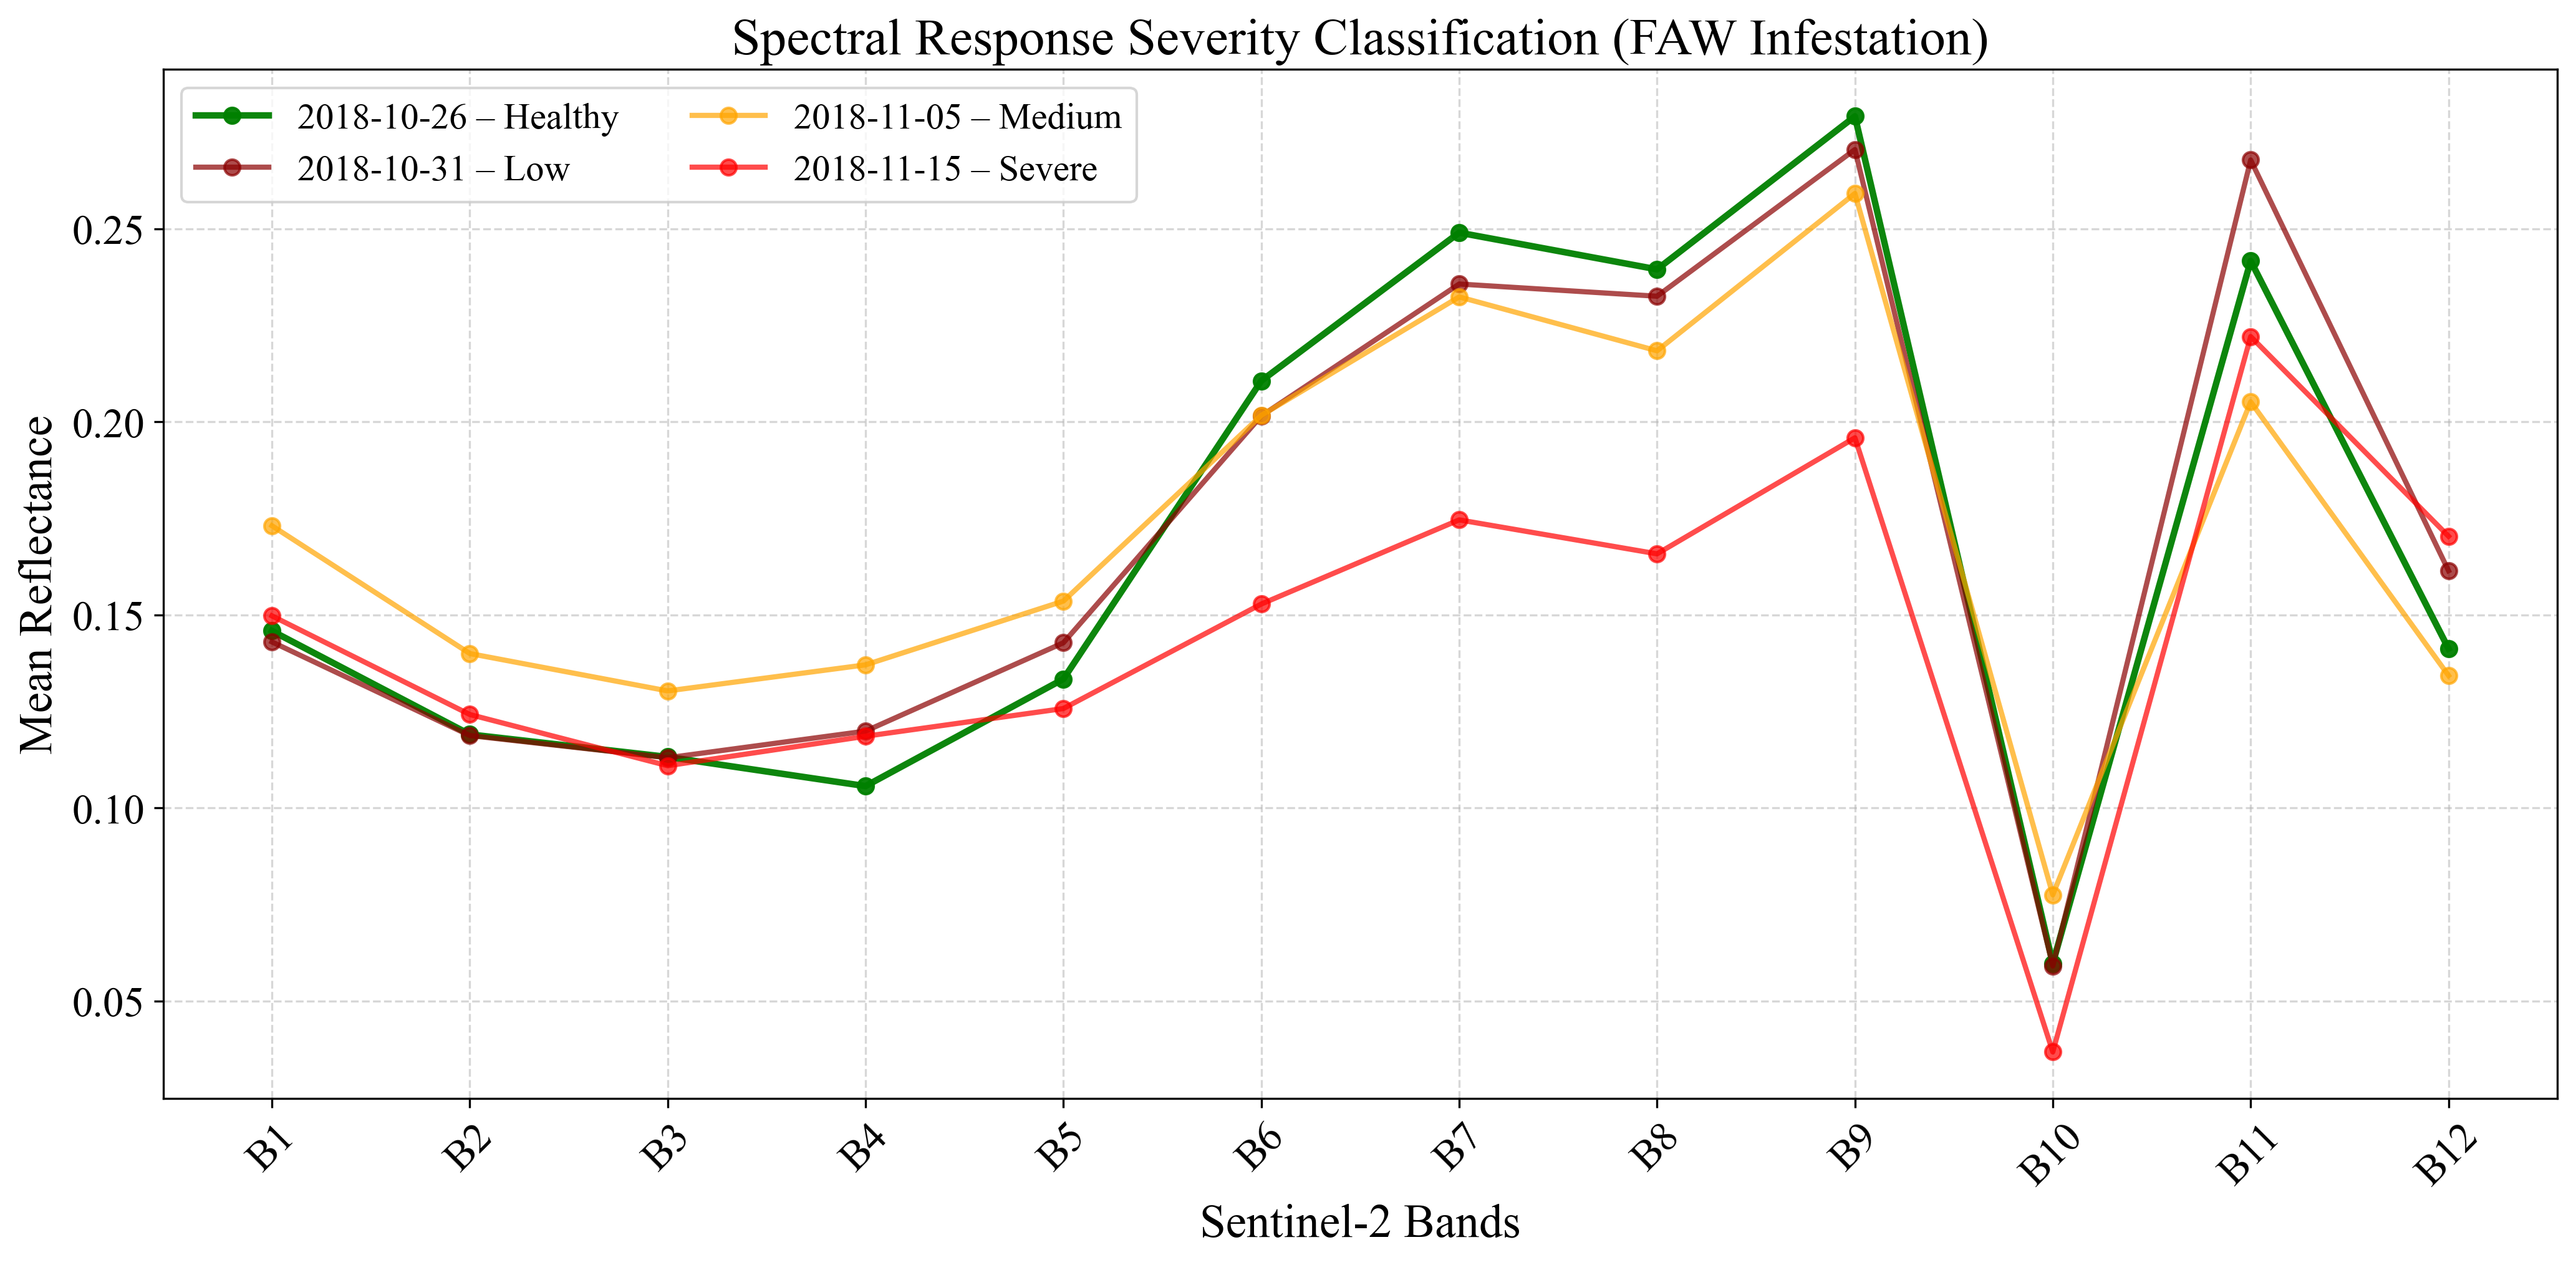
\includegraphics[width=1\textwidth]{figures/india_spectral_severity_classification.png}
                    \caption{Spectral signatures of maize crops under different severity levels of Fall Armyworm infestation in Southern India.}
                    \label{fig:india_spectral_severity_classification}
                \end{figure}
                \FloatBarrier

                Based on the mean spectral response of the field ilustrated in Figure \ref{fig:india_spectral_severity_classification},we can interpret the its results based on each spectral band characteristics. Near-Infrared (B8):carries information about leaf structure. Damage from pest feeding reduces reflectance in thisband. Blue (B2) and Red (B4) carry chlorophyll information. Chlorophyll absorbs these wavelengths;reduction in absorption indicates decreased photosynthetic activity, often caused by pestfeeding on leaves. Shortwave Infrared (B10-B12) are sensitive to water content.Pest-damaged plants often exhibit water stress, detectable in these bands.
 
                Harvest events cause abrupt transitions from high NDVI (green, healthy) to low NDVI  (senescence, yellow/brown), which must be distinguished from pest-related declines. Pest-related NDVI declines are more gradual and associated with specific temporal patterns linked to pest life cycles and feeding behavior.

            \subsubsection{NDVI Time-Series Analysis}

                Figure \ref{fig:2019indiaseries} present the NDVI time-series of the FAW-infested field in Southern India for the year of 2019, while Figure \ref{fig:2018indiaseries} shows the NDVI time-series of the same field for the year of 2018. The temporal patterns in these time-series reveal significant differences between the two years, particularly during the period of FAW infestation. In 2018, we observe a clear decline in NDVI values corresponding to the infestation period, indicating a reduction in vegetation health and biomass due to pest damage. In contrast, the 2019 time-series shows a more stable NDVI pattern, suggesting healthier vegetation conditions without significant pest-related stress. These observations highlight the potential of Sentinel-2 time-series analysis for monitoring crop health and detecting pest infestations in agricultural fields.

                \begin{figure}[!ht]
                    \centering
                    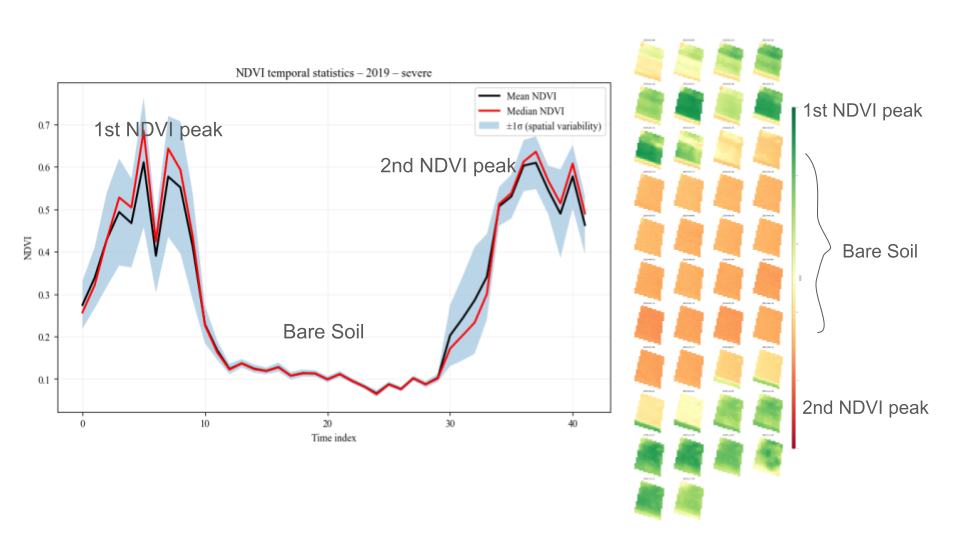
\includegraphics[width=0.8\textwidth]{figures/2019_india_timeseries.png}
                    \caption{NDVI time series of 2019 in Southern India.}
                    \label{fig:2019indiaseries}
                \end{figure}
                \FloatBarrier

                \begin{figure}[!ht]
                    \centering
                    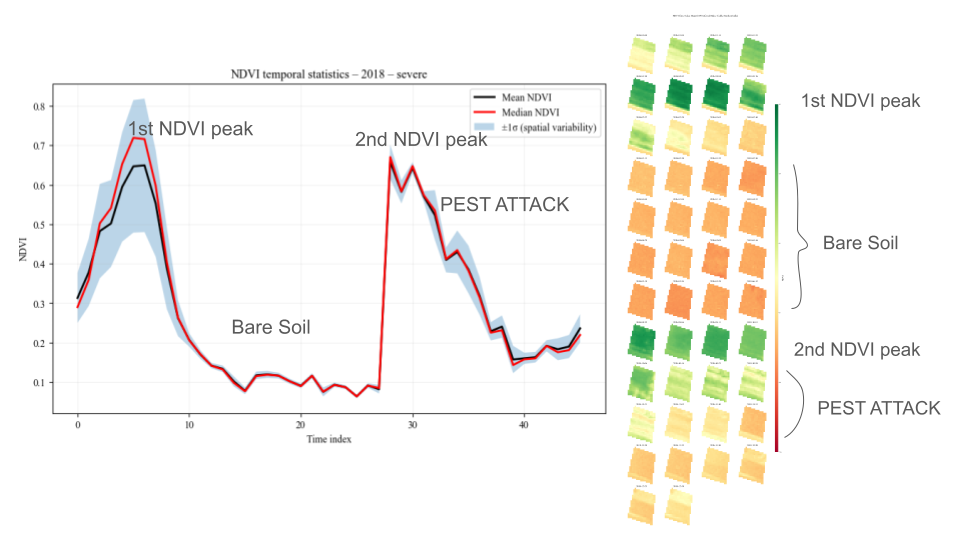
\includegraphics[width=0.8\textwidth]{figures/2018_india_timeseries.png}
                    \caption{NDVI time series of 2018 in Southern India.}
                    \label{fig:2018indiaseries}
                \end{figure}
                \FloatBarrier

                Figure \ref{fig:india_lai_time_series_maps} show the LAI time-series maps of the FAW-infested field in Southern India. We observe a clear temporal decline in LAI values across the field,corresponding to the period of FAW infestation. The spatial patterns in these maps highlight the extent and severity of the damage caused by the pest, with lower index values indicatingareas of more severe infestation and biomass loss.

                \begin{figure}[!ht]
                    \centering
                    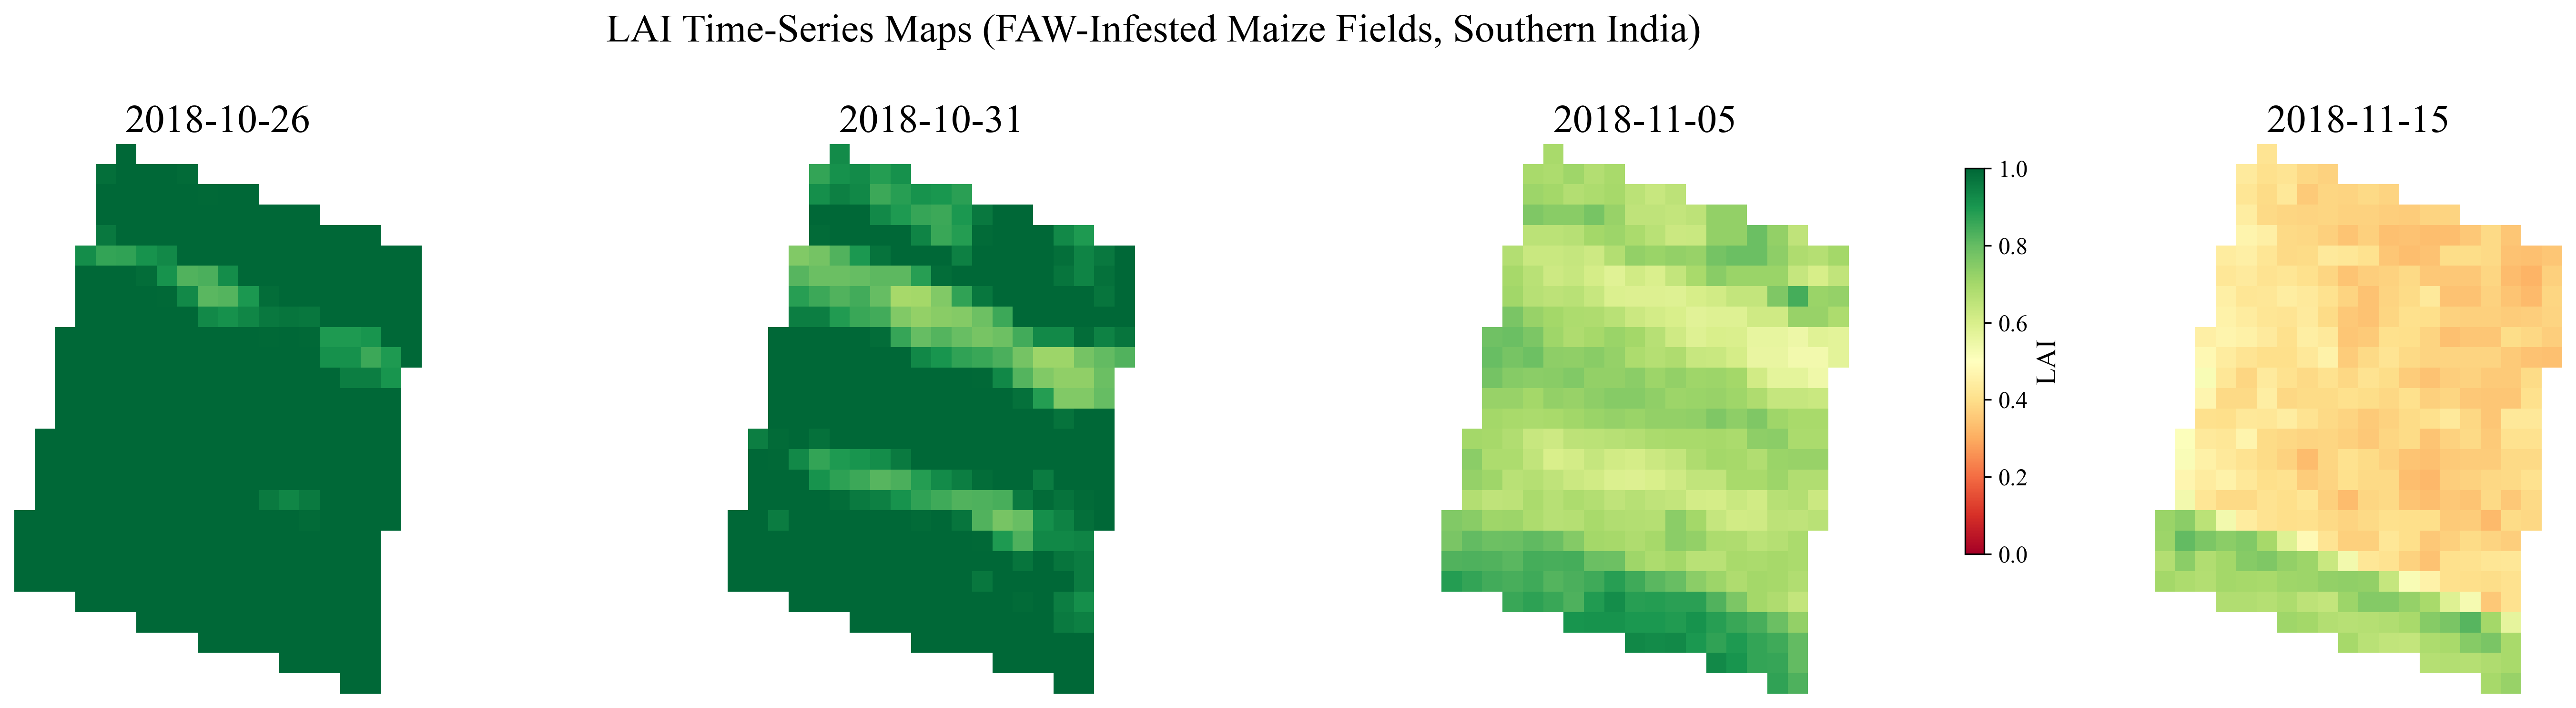
\includegraphics[width=1\textwidth]{figures/india_lai_time_series_maps.png}
                    \caption{LAI time series of FAW-infested in Southern India.}
                    \label{fig:india_lai_time_series_maps}
                \end{figure}
                \FloatBarrier

                Based on the results presented in Figures \ref{fig:2019indiaseries}, \ref{fig:2018indiaseries}, and \ref{fig:india_lai_time_series_maps}, we can conclude that Sentinel-2 time-series analysis is a valuable tool for monitoring crop health and detecting pest infestations. The observed decline in NDVI and LAI values during the FAW infestation period indicates significant stress on the vegetation, which can be effectively captured through remote sensing techniques. These findings underscore the potential of using satellite imagery for early detection of pest outbreaks, enabling timely interventions to mitigate crop damage and improve agricultural productivity.
        
            \subsection{FAW infestation detection in Ghana with Sentinel-2}

            In Ghana, we followed the study by \cite{bilintoh2019remote}, who performed field validation in Ejura between May and July 2018 to assess the Fall Armyworm (FAW) impact from the 2017 growing season (April to September). Specifically, we utilized his approach of combining remote sensing with statistical techniques to assess the uncertainty in factors related to infestation in maize. 

            However, as noted in the original work, the lack of specific dates for certain phenological stages or infestation events made the analysis difficult. This difficulty was compounded by gaps in the temporal resolution of satellite imagery and the presence of extensive cloud cover during the 2017 growing season, which limited the ability to capture the full maize phenological cycle as presented in Figure \ref{fig:extensive-cc}.

            \begin{figure}[!ht]
                \centering
                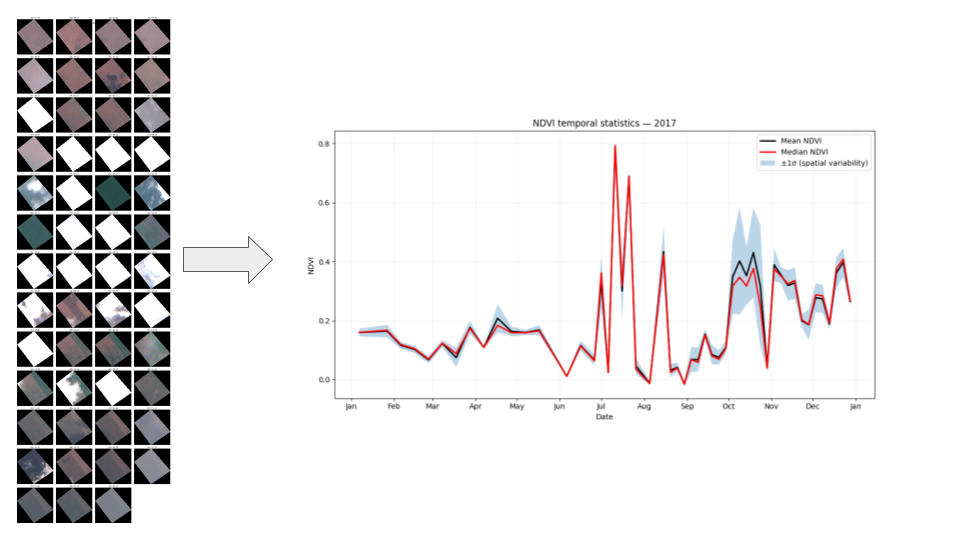
\includegraphics[width=0.8\textwidth]{figures/EXTENSIVE-CC.png}
                \caption{NDVI time series of 2017 in Ejura, Ghana, illustrating the sparse data availability due to cloud cover.}
                \label{fig:extensive-cc}
            \end{figure}
            \FloatBarrier

            \subsubsection{NDVI Time-Series Analysis}

            Figures \ref{fig:2019ghanaseries} and \ref{fig:2020ghanaseries} present the NDVI time-series for subsequent years. While these series offer better temporal coverage than the 2017 data, they highlight the persistent challenge of defining a "normal" maize profile in this region.

            \begin{figure}[!ht]
                \centering
                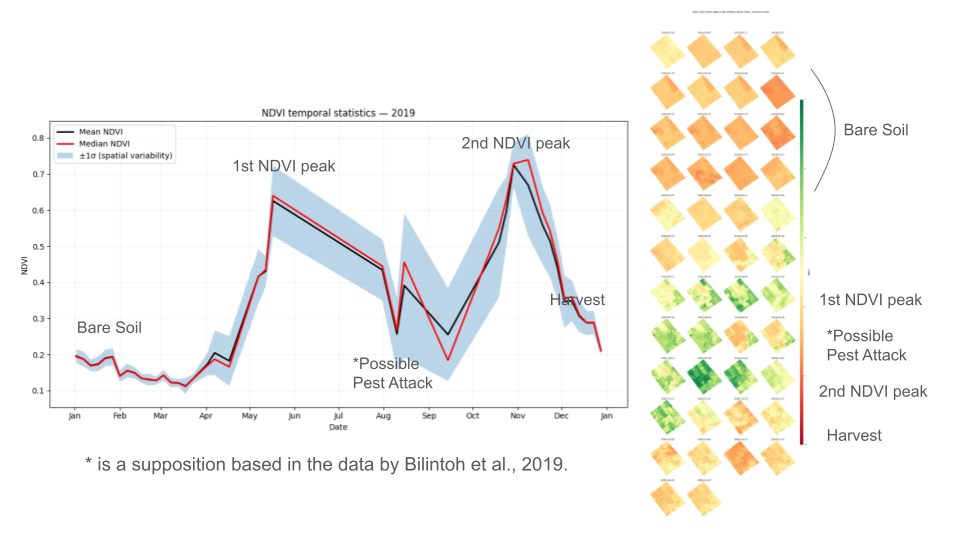
\includegraphics[width=0.8\textwidth]{figures/gh1.png}
                \caption{NDVI time series of 2019 in Ejura, Ghana.}
                \label{fig:2019ghanaseries}
            \end{figure}
            \FloatBarrier

            \begin{figure}[!ht]
                \centering
                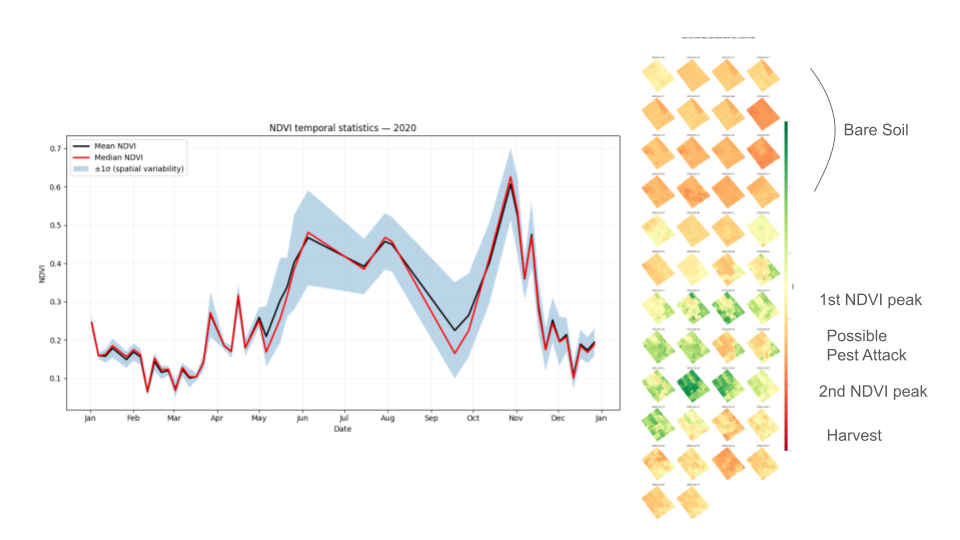
\includegraphics[width=0.8\textwidth]{figures/gh2.png}
                \caption{NDVI time series of 2020 in Ejura, Ghana.}
                \label{fig:2020ghanaseries}
            \end{figure}
            \FloatBarrier

            The interpretation of these spectral curves is further complicated by the heterogeneous nature of the farming landscape in Ejura. \cite{bilintoh2019remote} field surveys revealed that local farmers rarely maintain monoculture maize plots; instead, they practice complex intercropping and crop rotation. The analyzed fields contained a mixture of crops, including plantain, yam, rice, beans, cassava, groundnuts, and watermelon. Specifically, beans and groundnuts are frequently rotated with maize to maintain soil nitrogen levels. 

            This mixture of crop types, each with distinct phenological timings and greenness peaks, creates a "mixed-pixel" effect in the Sentinel-2 data. Consequently, the observed growth cycles deviate significantly from standard maize models, as the integrated spectral signature reflects multiple overlapping stages of planting and harvesting. This agricultural diversity, coupled with the lack of precise infestation timestamps, necessitates a robust univariate analysis capable of distinguishing between pest-induced stress and the inherent noise of intercropped vegetation dynamics.

        \section{Application Development}
            In parallel to the RSAD modeling, I participated in app development testing and remote sensing model integration for the PEZEGO pest-management app. This experience provided insights into scalable application design, optimization techniques, and model deployment strategies, which can be applied to enhance our ongoing project, GeoHuman. The PEZEGO app focuses on providing actionable insights to farmers for pest management, and my involvement in this project allowed me to contribute to the development of user-friendly interfaces and efficient data processing pipelines.

\section{Conclusion}

This research internship demonstrated the potential of RSAD using Sentinel-2 time-series to identify pest-induced stress in agricultural systems. The case study in Southern India validated the approach, as NDVI and LAI declines aligned with documented FAW infestation periods, confirming that vegetation indices can capture meaningful stress signals.
In contrast, experiments in Ejura, Ghana, revealed key limitations in real-world settings. Persistent cloud cover, irregular temporal sampling, and complex intercropping reduced the separability between normal phenological variation and anomalies. These challenges highlight the limitations of univariate approaches and the need for more robust representations.

From a methodological perspective, this work shows that while univariate time-series analysis can serve as a lightweight and interpretable baseline for RSAD, it is insufficient for operational deployment in diverse agricultural landscapes. The primary bottleneck is not only model capacity, but data quality and contextual ambiguity, particularly in the absence of synchronized ground-truth observations. Consequently, anomaly attribution remains uncertain, as deviations may result from multiple confounding factors such as harvesting cycles, water stress, or mixed-pixel effects.

Overall, this work establishes a proof of concept for RSAD in agricultural monitoring while clearly identifying its current limitations. More importantly, it defines a structured pathway toward operational systems by emphasizing the joint need for (i) richer multimodal data representations and (ii) reliable ground-truth acquisition pipelines. These components are essential to move from exploratory analysis to real-world decision tools in agriculture.

\section{Future Work}

\begin{itemize}
    \item \textbf{Plasticulture Application:} The RSAD techniques refined during this period will be further explored in the context of plasticulture in Brazil, specifically to monitor material deterioration and the subtle spectral shifts associated with the use of protective netting.
    \item \textbf{Multivariate Time-Series Integration:} Future work should transition from univariate analysis to Multivariate Time-Series (MTS) representations. By simultaneously monitoring multiple spectral indices (e.g., NDVI, EVI, and NDWI) along with SAR (Synthetic Aperture Radar) data, models can better differentiate between water stress, harvesting, and pest damage, significantly reducing false-positive rates.
    \item \textbf{Ground-Truth Data Collection:} To move beyond a proof of concept, future efforts must prioritize the collection of date-stamped field surveys. Integrating the GeoHuman and PEZEGO applications to collect real-time farmer observations will be crucial for creating the labeled datasets necessary to validate and train supervised anomaly detection models.
    \item \textbf{Advanced Machine Learning Architectures:} Exploring more complex deep learning architectures, such as Graph Neural Networks (GNNs) or Transformers with Attention Mechanisms, could provide better solution of the problem, combining temporal and spatial dependencies of the data.
\end{itemize}

\section{Internship Experience}

    During the internship, Prof.\ Jefersson organized weekly seminars for the Computer Vision Research Group, where students presented their work or relevant research topics. I contributed by presenting my research ideas and discussing them with the group (Figure~\ref{fig:bites}), receiving valuable feedback that helped refine my approach. These seminars also provided the opportunity to learn a wide range of methodologies and perspectives from different research topics, further enriching my understanding of computer vision and machine learning.

    \begin{figure}[!ht]
        \centering
        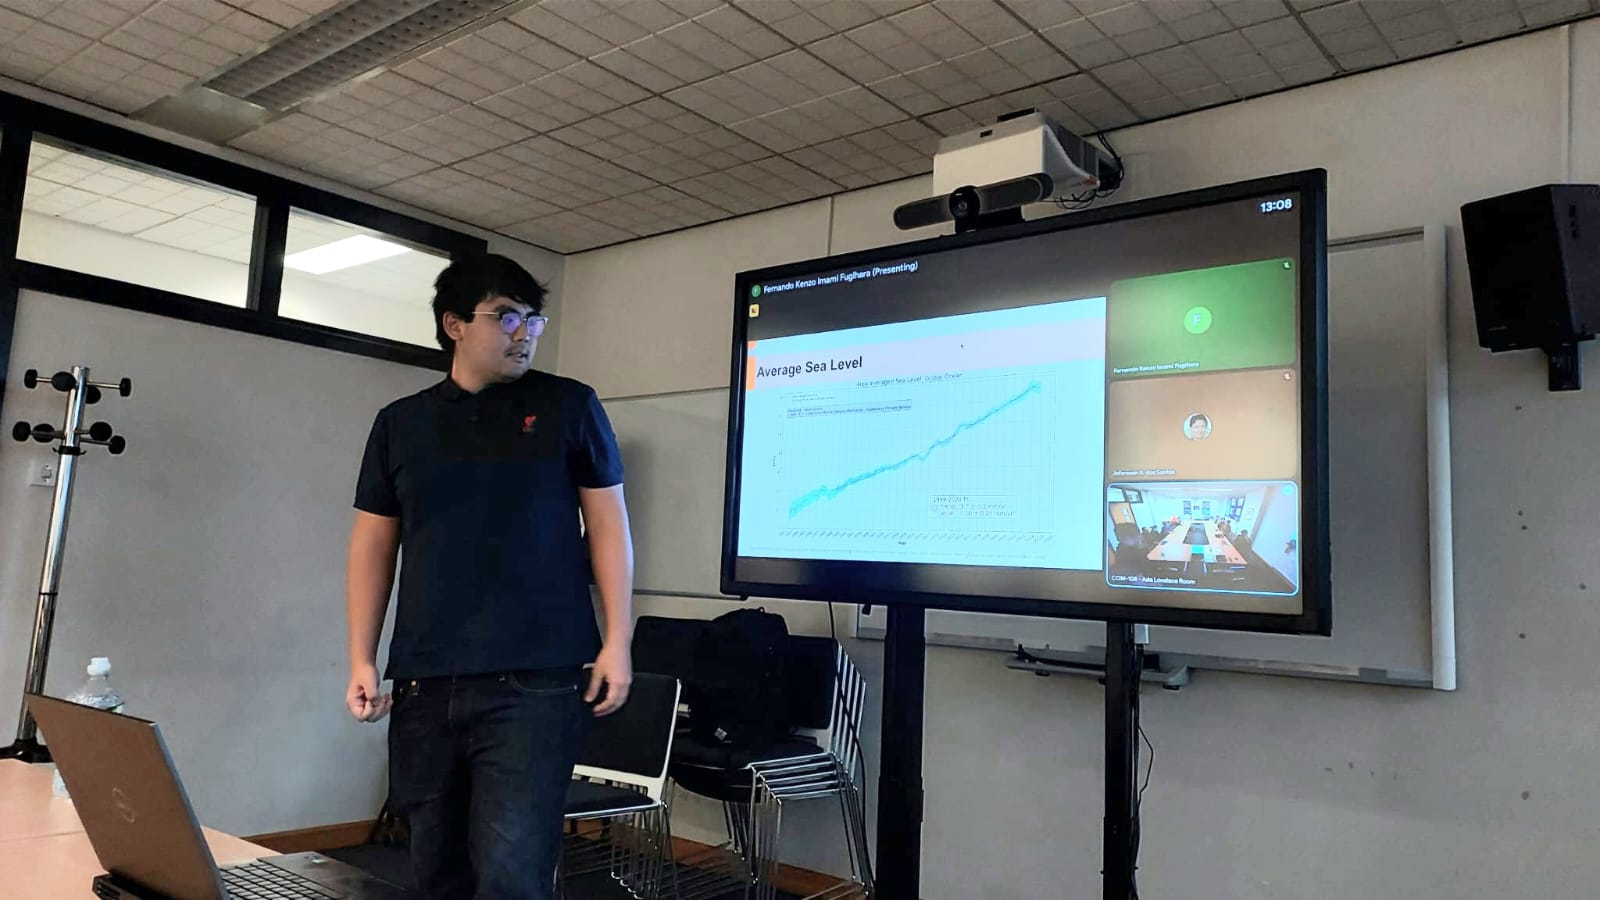
\includegraphics[width=0.7\textwidth]{figures/presenting.jpeg}
        \caption{Presenting my project results in a weekly seminar for the Computer Vision Group at the University of Sheffield.}
        \label{fig:bites}
    \end{figure}
    \FloatBarrier

    I also participated in meetings and workshops with the Pervasive Computing Research Group led by Prof. Po Yang, focused on the “SmartPest-Ghana: Exploring LLM-driven mobile solutions for climate-smart pest management in maize farming” project (for more information, visit \url{https://iuk-business-connect.org.uk/smartpest-ghana/}). This collaborative initiative involves the University of Sheffield, the University of Ghana, and UNICAMP. During these meetings, each member presented their progress and discussed potential solutions and research directions. These interactions were particularly valuable, as the multi-institutional nature of the project provided a wealth of different ideas and interdisciplinary insights. Engaging with experts from different regions allowed me to understand the unique challenges of West African agriculture, significantly broadening my research horizon. Figure~\ref{fig:presghana} shows my presentation to the research groups.

    \begin{figure}[!ht]
        \centering
        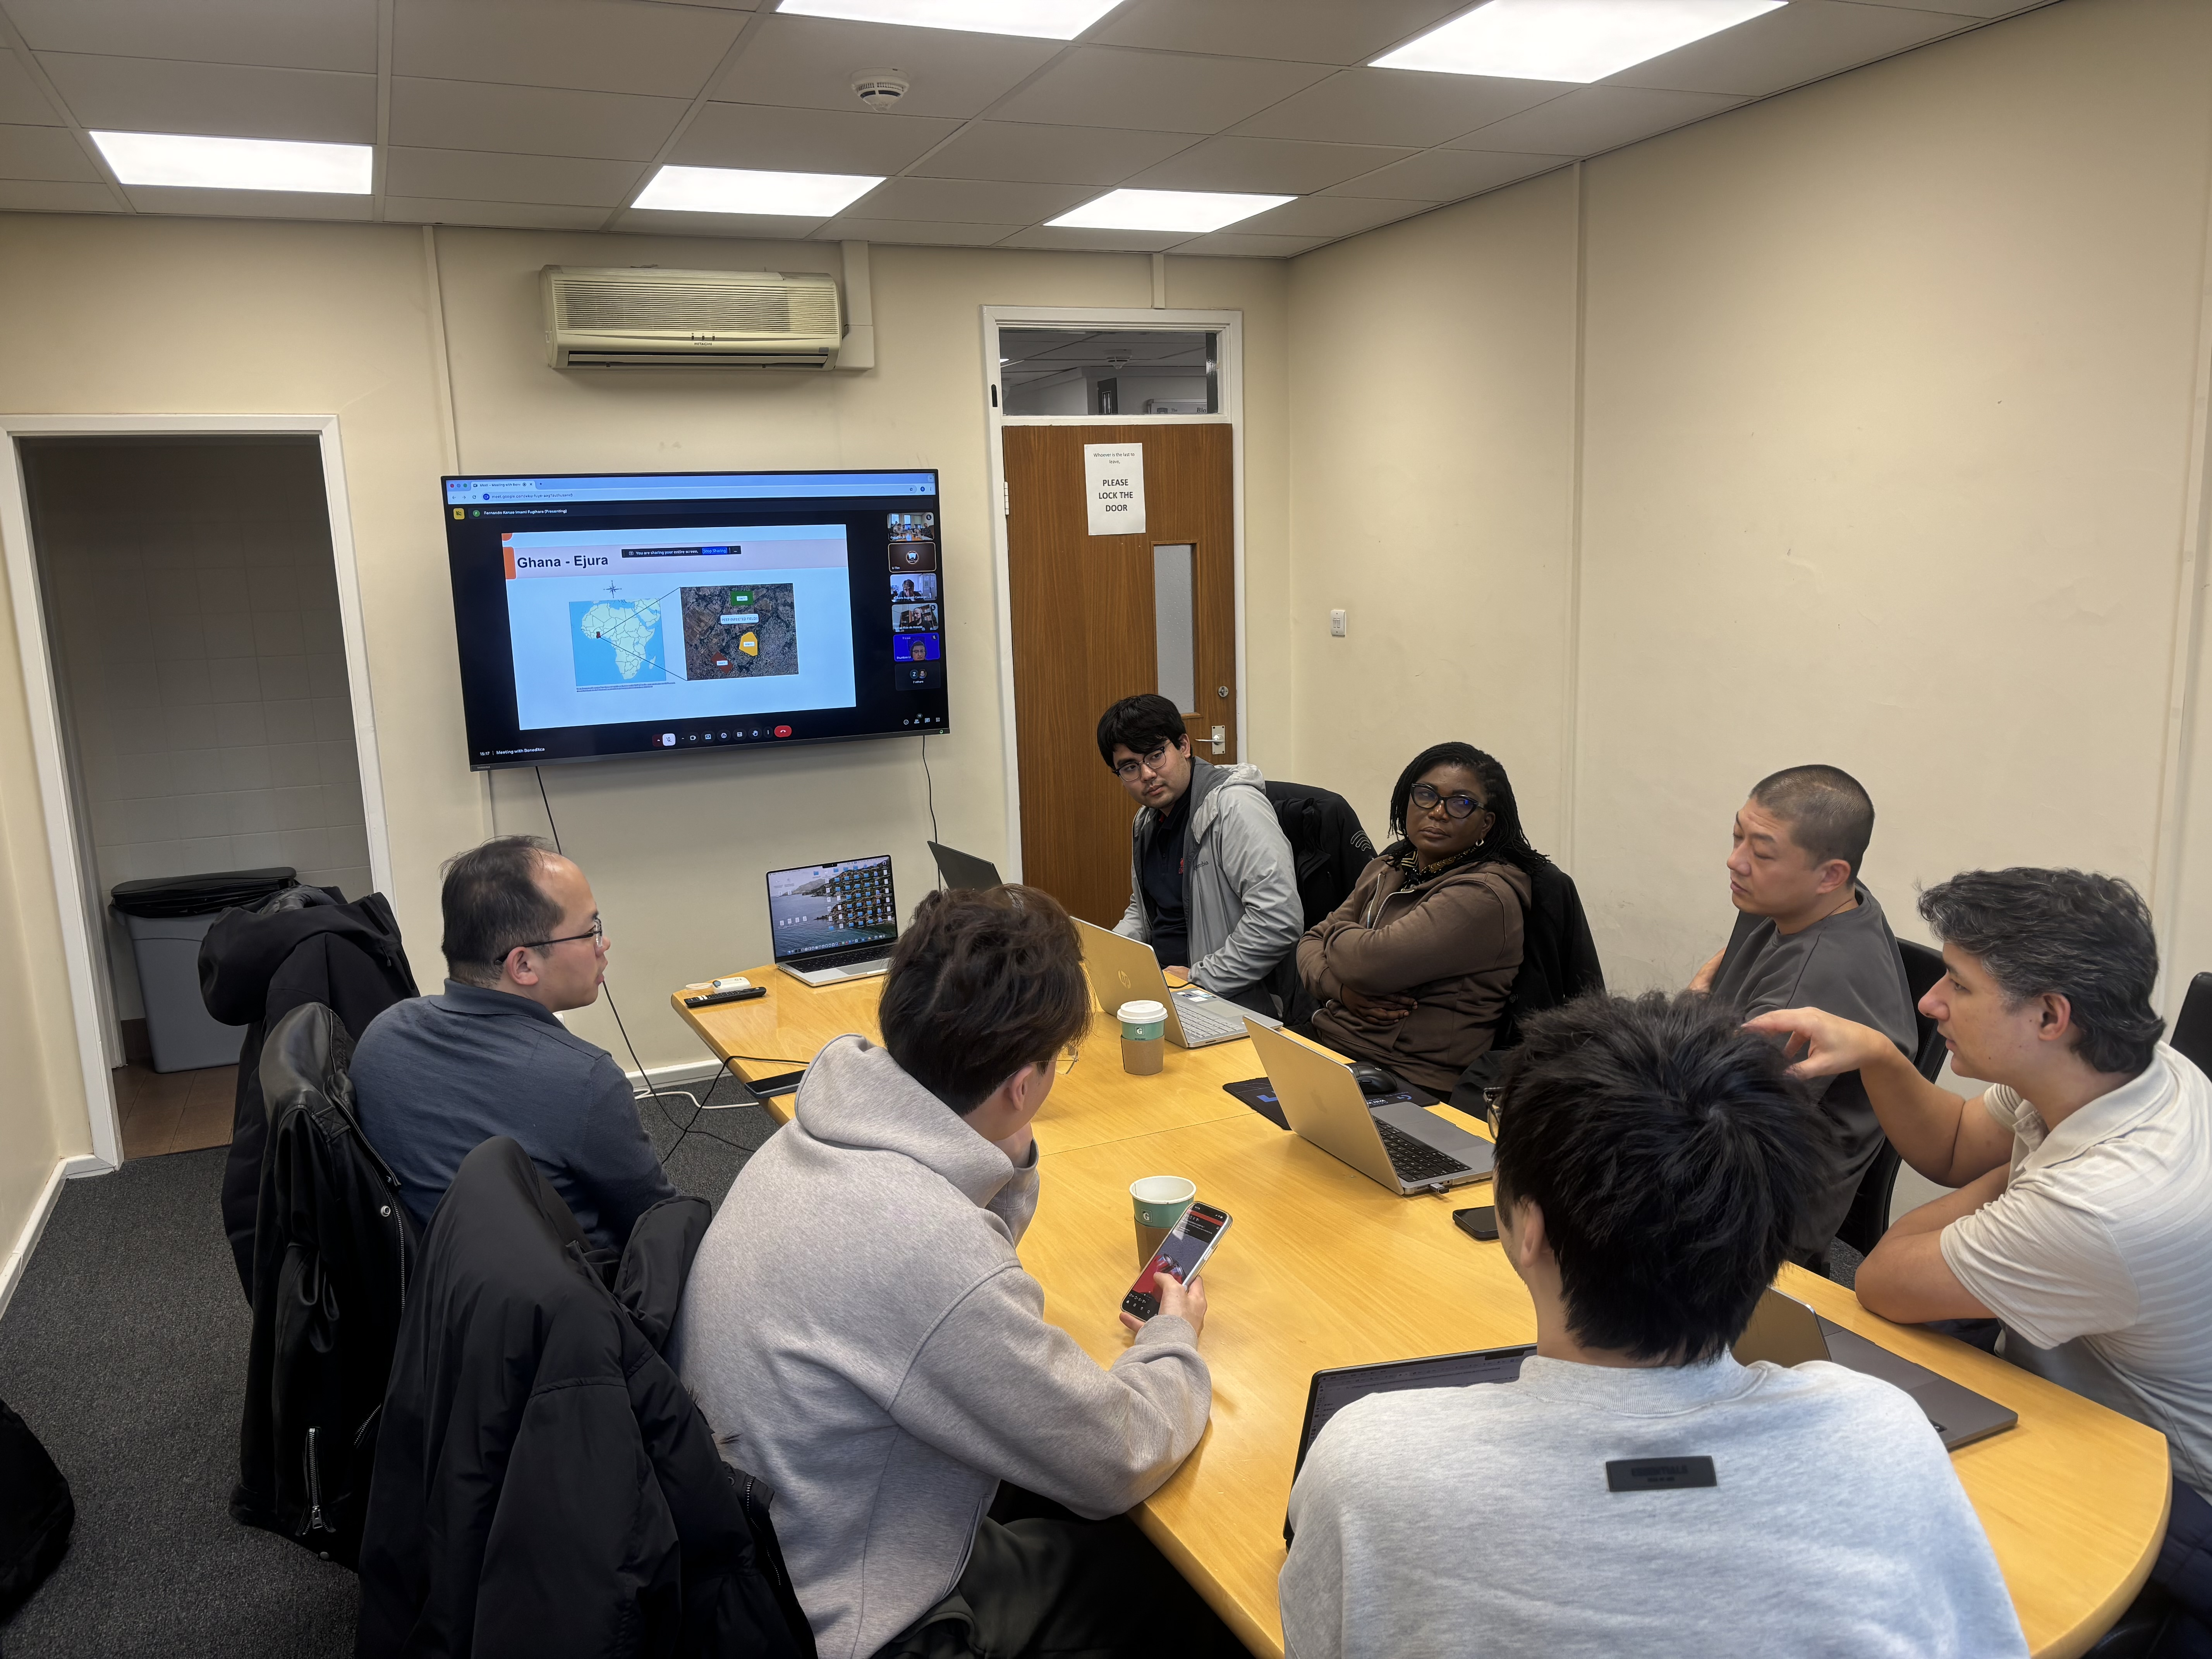
\includegraphics[width=0.7\textwidth]{figures/meeting.jpeg}
        \caption{Presenting my project results in a weekly seminar for the Pervasive Computing Group at the University of Sheffield.}
        \label{fig:presghana}
    \end{figure}
    \FloatBarrier

    The exchange program significantly enhanced my technical skills while profoundly enriching my personal life. Beyond the academic and research achievements, this experience expanded my horizons, exposing me to a diverse array of perspectives and global cultures. Engaging with researchers and students from different backgrounds fostered a new level of cultural awareness and intellectual openness that I will carry with me for the rest of my life.


\clearpage
\bibliography{kenzo}
\bibliographystyle{kenzo}
\clearpage

\appendix
\counterwithin{figure}{section}
\counterwithin{table}{section}
\counterwithin{equation}{section}

\section{Appendix}
\subsection{Time-Series Smoothing Techniques}
\label{appendix1}

        Smoothing techniques are essential preprocessing steps that remove noise from time-series data while preserving important patterns. This is particularly critical when comparing pixel time-series or applying distance-based algorithms.

        Consider two pixels with similar underlying patterns but different noise characteristics. Without smoothing, distance-based clustering algorithms may incorrectly classify these pixels as dissimilar due to noise rather than genuine differences in behavior. Smoothing addresses this issue by enhancing signal-to-noise ratio.

        The choice of smoothing method depends on the structural characteristics of the time-series, as summarized in Table \ref{tab:t1}.

        \begin{table}[h]
        \centering
        \caption{Smoothing algorithm applicability for different time-series structures}
        \label{tab:t1}
        \renewcommand{\arraystretch}{1.3}
            \begin{tabular}{|l|c|c|c|c|}
            \hline
            \textbf{Algorithm} & \textbf{Level} & \textbf{Trend} & \textbf{Seasonality} & \textbf{Parameters} \\
            \hline
            Single HWES  & Yes & No  & No  & $\alpha$ \\
            Double HWES  & Yes & Yes & No  & $\alpha, \beta$ \\
            Triple HWES  & Yes & Yes & Yes & $\alpha, \beta, \gamma$ \\
            \hline
            \end{tabular}
        \end{table}

        Table \ref{tab:t2} defines the variables used in smoothing formulations.

        \begin{table}[h]
        \centering
        \caption{Variables utilized in smoothing models}
        \label{tab:t2}
        \renewcommand{\arraystretch}{1.4}
            \begin{tabular}{|c|l|}
            \hline
            \textbf{Symbol} & \textbf{Description} \\
            \hline
            $X$ & Observation \\
            $S$ & Smoothed observation \\
            $B$ & Trend factor \\
            $C$ & Seasonal index \\
            $F$ & Forecast at $m$ periods ahead \\
            $\alpha$ & Data smoothing factor, $\alpha \in (0,1)$ \\
            $\beta$ & Trend smoothing factor, $\beta \in (0,1)$ \\
            $\gamma$ & Seasonal change smoothing factor, $\gamma \in (0,1)$ \\
            $\phi$ & Damped smoothing factor, $\phi \in (0,1)$ \\
            $t$ & Time period index \\
            \hline
            \end{tabular}
        \end{table}

        \subsubsection{Moving Average and Weighted Average}
            These methods compute the future value as the average (or weighted average) of $k$ previous values. While useful for trend observation and feature engineering, these approaches are unsuitable for satellite time-series with trend and seasonality components.

        \subsubsection{Single Exponential Smoothing (SES)}
            SES models the level component only and is appropriate for stationary series without trend or seasonality. It weights recent observations more heavily based on the assumption that the future is more closely related to the recent past.

            \[
                S_0 = X_0
            \]

            \[
                S_t = \alpha X_t + (1 - \alpha) S_{t-1}, \quad t > 0, \; 0 < \alpha < 1
            \]

            \textbf{Application:} Limited applicability to agricultural time-series, which typically exhibit both trend and seasonality.

        \subsubsection{Double Exponential Smoothing (DES)}
            DES extends SES by incorporating trend, making it suitable for series with trend but without seasonality.

            \[
                \begin{aligned}
                S_0 &= X_0 \\
                B_0 &= X_1 - X_0 \\
                S_t &= \alpha X_t + (1 - \alpha)(S_{t-1} + B_{t-1}) \\
                B_t &= \beta (S_t - S_{t-1}) + (1 - \beta) B_{t-1}, \quad \alpha, \beta \in (0,1)
                \end{aligned}
            \]

            \textbf{Application:} Applicable to agricultural time-series when seasonality is not a dominant factor.

        \subsubsection{Triple Exponential Smoothing (TES)}
            TES represents the most comprehensive smoothing approach, modeling level, trend, and seasonality simultaneously. This method is most appropriate for agricultural satellite time-series, which exhibit all three components.

            \[
                \begin{aligned}
                S_0, F_0 &= X_0 \\
                B_0 &= \frac{\sum_{i=0}^{L-1} \left( X_{L+i} - X_i \right)}{L^2} \\
                S_t &= \alpha \left( X_t - C_{t \bmod L} \right) + (1 - \alpha)\left( S_{t-1} + \phi B_{t-1} \right) \\
                B_t &= \beta \left( S_t - S_{t-1} \right) + (1 - \beta)\phi B_{t-1} \\
                C_{t \bmod L} &= \gamma \left( X_t - S_t \right) + (1 - \gamma) C_{t \bmod L} \\
                F_{t+m} &= S_t + B_t \sum_{i=1}^{m} \phi^{i} + C_{t \bmod L}, \quad \alpha, \beta, \gamma \in (0,1)
                \end{aligned}
            \]

            \textbf{Application:} Recommended for Sentinel-2 vegetation index time-series, which exhibit clear seasonal patterns related to crop phenology.

\end{document}
